\documentclass[11pt,a4paper]{article}

% --- Geometry & spacing ----------------------------------------------------
\usepackage[a4paper, margin=1in, top=1.1in, bottom=1.1in]{geometry}
\usepackage{microtype}
\usepackage{setspace}
\setstretch{1.18}
\setlength{\parskip}{0.5\baselineskip}
\setlength{\parindent}{0pt}

% --- Typography ------------------------------------------------------------
\usepackage[T1]{fontenc}
\usepackage[utf8]{inputenc}
\usepackage{lmodern}
\usepackage{textcomp}

% --- Colour ----------------------------------------------------------------
\usepackage{xcolor}
\definecolor{ink1}{HTML}{0a0a0a}      % near black
\definecolor{ink2}{HTML}{1f1f1f}      % body text
\definecolor{ink3}{HTML}{555555}      % muted
\definecolor{accent}{HTML}{0d8a72}    % editorial teal (PDF readable)
\definecolor{accentSoft}{HTML}{e8f4f1}
\definecolor{warn}{HTML}{c47a09}
\definecolor{bad}{HTML}{a83232}
\definecolor{ok}{HTML}{2f7a4d}
\definecolor{rule}{HTML}{cccccc}
\definecolor{coverInk}{HTML}{0a0a0a}
\definecolor{coverPaper}{HTML}{f5efe6}

% --- Lists, tables, links --------------------------------------------------
\usepackage{enumitem}
\setlist[itemize]{leftmargin=1.4em, itemsep=2pt, topsep=4pt}
\setlist[enumerate]{leftmargin=1.6em, itemsep=2pt, topsep=4pt}
\usepackage{booktabs}
\usepackage{array}
\usepackage{longtable}
\usepackage{multicol}
\usepackage{tabularx}
\usepackage{ltablex}
\keepXColumns
\usepackage[hidelinks, colorlinks=true, linkcolor=accent, urlcolor=accent, citecolor=accent]{hyperref}

% --- Section formatting ----------------------------------------------------
\usepackage{titlesec}
\titleformat{\section}
  {\color{ink1}\Large\bfseries}{\thesection}{0.65em}{}
\titleformat{\subsection}
  {\color{accent}\large\bfseries}{\thesubsection}{0.55em}{}
\titleformat{\subsubsection}
  {\color{ink2}\normalsize\bfseries}{\thesubsubsection}{0.5em}{}
\titlespacing*{\section}{0pt}{1.6em}{0.7em}
\titlespacing*{\subsection}{0pt}{1.0em}{0.4em}

% --- Headers & footers -----------------------------------------------------
\usepackage{fancyhdr}
\pagestyle{fancy}
\fancyhf{}
\renewcommand{\headrulewidth}{0.4pt}
\renewcommand{\footrulewidth}{0pt}
\fancyhead[L]{\color{ink3}\footnotesize\textsc{DataLens AI {\textbar} System Whitepaper}}
\fancyhead[R]{\color{ink3}\footnotesize\thepage}
\fancyfoot[C]{\color{ink3}\footnotesize \today}

% --- Boxes for callouts ----------------------------------------------------
\usepackage[most]{tcolorbox}
\tcbset{
  colback=accentSoft,
  colframe=accent,
  boxrule=0.4pt,
  arc=2pt,
  left=8pt, right=8pt, top=4pt, bottom=4pt,
  fonttitle=\bfseries\color{ink1}
}

% --- Code listings ---------------------------------------------------------
\usepackage{listings}
\lstdefinestyle{ds}{
  basicstyle=\ttfamily\footnotesize,
  backgroundcolor=\color{accentSoft},
  frame=single,
  rulecolor=\color{accent},
  keywordstyle=\color{accent}\bfseries,
  stringstyle=\color{warn},
  commentstyle=\color{ink3}\itshape,
  numbers=left,
  numberstyle=\color{ink3}\tiny,
  numbersep=8pt,
  breaklines=true,
  showstringspaces=false,
  language=Python,
  tabsize=2,
}
\lstset{style=ds}

% --- Figures ---------------------------------------------------------------
\usepackage{graphicx}
\usepackage{caption}
\captionsetup{font={small,it},labelfont={bf,color=accent},skip=4pt}
\usepackage{subcaption}

% --- TikZ for the architecture diagram ------------------------------------
\usepackage{tikz}
\usetikzlibrary{shapes.geometric, arrows.meta, positioning, fit, backgrounds}

% --- Title page macros -----------------------------------------------------
\newcommand{\eyebrow}[1]{{\color{accent}\fontfamily{cmtt}\selectfont\small\MakeUppercase{#1}}}

\title{\vspace{-2em}\Huge\bfseries DataLens AI \\[0.2em] {\Large System Whitepaper \& Component Audit}}
\author{Compiled automatically from live test runs}
\date{\today}

\begin{document}


\thispagestyle{empty}

\begin{flushleft}
\eyebrow{DataLens AI \quad{$\boldsymbol{\cdot}$}\quad System Whitepaper}

\vspace{1.2em}
{\fontsize{42}{52}\selectfont\bfseries Inside\,DataLens.}

\vspace{0.4em}
{\fontsize{20}{26}\selectfont\color{accent}\bfseries Architecture, methods,}\\[2pt]
{\fontsize{20}{26}\selectfont\color{accent}\bfseries and a live component audit.}

\vspace{1.6em}
{\large\color{ink2} A walkthrough of every analytical module in the project,
the algorithms it relies on, and what each one produced when exercised against
3 representative datasets.}

\vspace{2em}

\begin{tabularx}{\linewidth}{X X X X}
\toprule
\textsc{Datasets} & \textsc{Components} & \textsc{Pass} & \textsc{Pass\,rate} \\
\midrule
3 & 72 & 72 & 100.0\% \\
\bottomrule
\end{tabularx}

\vfill

{\color{ink3}\footnotesize Generated May 24, 2026
{\quad$\boldsymbol{\cdot}$\quad}
Manifest: \texttt{reports/component\_test\_manifest.json}
{\quad$\boldsymbol{\cdot}$\quad}
Builder: \texttt{tools/whitepaper\_builder.py}}
\end{flushleft}

\newpage


\section*{Abstract}
\addcontentsline{toc}{section}{Abstract}

DataLens AI is a Python-first analytical pipeline that turns an arbitrary
tabular dataset into a complete dashboard, a typeset PDF report, and a
chat-style question-answering interface, all without the user having to
write code. This whitepaper documents how it works, end to end, with two
goals in mind. First, to give a self-contained explanation of every
analytical module --- what it computes, why that computation matters, and
which classical algorithm it sits on top of. Second, to back those
explanations with a live audit: every module described here was exercised
against three representative datasets just before this document was
generated, and the empirical evidence (timings, summary metrics, and any
failures) is included verbatim.

The audience for this document is anyone who wants to understand DataLens
deeply enough to trust it: a stakeholder evaluating its outputs, an
engineer debugging or extending it, or a reviewer assessing whether its
methodology is sound. We have therefore traded brevity for clarity: each
chapter starts with a primer on the underlying concepts (e.g.\ what SHAP
values are and what they are useful for) before showing the live results.

\noindent\textbf{Reproducibility note.} Re-running
\texttt{python tools/component\_test.py} regenerates the manifest;
re-running \texttt{python tools/whitepaper\_builder.py} regenerates this PDF.

\newpage
\tableofcontents
\newpage


\section{Introduction}

DataLens has a deliberately uncluttered shape. A dataset arrives at
\texttt{POST /api/analyze}; in $\sim 5$--$15$ seconds a fully-analysed JSON
payload comes back, populated with everything the dashboard needs and a
\texttt{downloadLinks.report} URL pointing at a generated PDF. Every step in
between is a small, individually-testable Python module.

This whitepaper is structured as follows. Section~\ref{sec:arch} covers the
overall architecture --- the orchestrator, parallelism, and how phases share
state. Sections~\ref{sec:ingest}--\ref{sec:agentic} each pair a methods
primer with the live evidence emitted by the corresponding module(s) when
they were last exercised. Section~\ref{sec:timings} aggregates timing
budgets across the test datasets. Section~\ref{sec:limits} is honest about
what the project does \emph{not} do well today.

The live evidence in this document came from
\texttt{3} datasets:
classification, regression, no\_target.


\section{System Architecture}\label{sec:arch}

\subsection{Top-down view}

DataLens is a single-process Flask backend that runs an analytical pipeline,
plus a Vite-served React dashboard. The two communicate over a stable JSON
contract. There is no database --- every analysis lives in an in-memory cache
keyed by a per-run \texttt{dataset\_id} and is regenerated on demand.

\begin{figure}[h!]
\centering
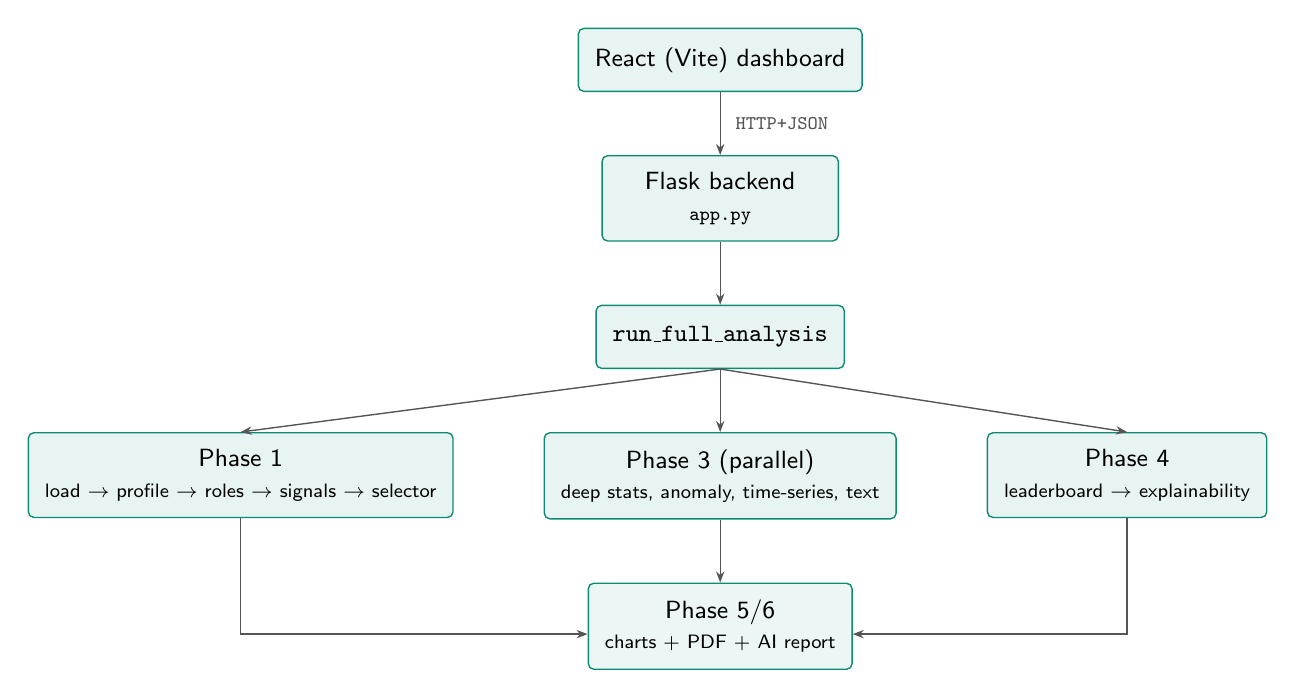
\begin{tikzpicture}[
  font=\small\sffamily,
  node distance=8mm and 12mm,
  every node/.style={align=center},
  block/.style={rectangle, draw=accent, fill=accentSoft, line width=0.5pt,
    rounded corners=2pt, inner sep=6pt, minimum width=30mm, minimum height=8mm},
  layer/.style={rectangle, draw=ink3!40, dashed, line width=0.4pt,
    rounded corners=2pt, inner sep=8pt, fill=none},
  arrow/.style={-{Stealth[length=4pt]}, line width=0.5pt, color=ink3},
]
  \node[block] (react) {React (Vite) dashboard};
  \node[block, below=of react] (flask) {Flask backend \\ {\scriptsize\ttfamily app.py}};
  \node[block, below=of flask] (orch) {\texttt{run\_full\_analysis}};

  \node[block, below left=of orch, xshift=-6mm] (p1) {Phase 1 \\ {\scriptsize load $\rightarrow$ profile $\rightarrow$ roles $\rightarrow$ signals $\rightarrow$ selector}};
  \node[block, below=of orch] (p3) {Phase 3 (parallel) \\ {\scriptsize deep stats, anomaly, time-series, text}};
  \node[block, below right=of orch, xshift=6mm] (p4) {Phase 4 \\ {\scriptsize leaderboard $\rightarrow$ explainability}};

  \node[block, below=of p3, fill=accent!8] (out) {Phase 5/6 \\ {\scriptsize charts $+$ PDF $+$ AI report}};

  \draw[arrow] (react) -- node[right=2pt, font=\scriptsize\ttfamily, color=ink3] {HTTP+JSON} (flask);
  \draw[arrow] (flask) -- (orch);
  \draw[arrow] (orch.south) -- (p1.north);
  \draw[arrow] (orch.south) -- (p3.north);
  \draw[arrow] (orch.south) -- (p4.north);
  \draw[arrow] (p3) -- (out);
  \draw[arrow] (p1.south) |- ([yshift=-1mm]out.west);
  \draw[arrow] (p4.south) |- ([yshift=-1mm]out.east);
\end{tikzpicture}
\caption{High-level pipeline. A request travels from the React dashboard through
\texttt{app.py} into \texttt{run\_full\_analysis}, which fans out across the
six phases. Phase 3 runs in parallel via a \texttt{ThreadPoolExecutor}; the
other phases are sequential because they either share state or rely on
matplotlib (which is not thread-safe).}
\label{fig:architecture}
\end{figure}

\subsection{Phase orchestration}

The orchestrator is \texttt{modules/pipeline.py:run\_full\_analysis()}. It
runs in six phases, with two important properties. First, every phase is
\emph{wrapped} in \texttt{\_safe\_call()} which converts any exception into a
JSON-safe error dict --- a single failing module cannot sink the run. Second,
phases that are pure-compute and independent are run in parallel using a
\texttt{ThreadPoolExecutor} (default 4 workers); phases that are sequential
or matplotlib-bound are not. The full timing breakdown is returned in
\texttt{result["timings\_ms"]} and visualised in the dashboard.


\section{Ingest --- understanding the dataset}\label{sec:ingest}

The first job of a data-analysis pipeline is to figure out what kind of data it is looking at. DataLens does this in five short, sequential phases: load, profile, role inference, signal detection, and analysis selection.

\textbf{Loading} normalises raw bytes into a \texttt{pandas.DataFrame}. The loader handles CSV, TSV, Excel and JSON formats, sniffs separators, and tolerates BOMs. It is intentionally tolerant --- bad rows are dropped with a warning rather than crashing the run.

\textbf{Profiling} captures the structural footprint of the dataset: shape, dtypes, per-column missing counts, per-column dtype histograms, sample of the head/tail, duplicate-row count, and cardinality. This is the cheapest and most general view, and almost every downstream module reads from it.

\textbf{Column role inference} assigns multi-label tags to each column (\texttt{numeric}, \texttt{categorical\_low}, \texttt{id\_like}, \texttt{price\_like}, \texttt{volume\_like}, \texttt{boolean}, \texttt{datetime\_like}, \texttt{long\_text}, etc.) using a mix of dtype inspection, name regexes (\texttt{price}, \texttt{revenue}, \texttt{id}, \texttt{date}), cardinality ratios and content sniffing. Roles are what allow the chart planner and the auto-cleaner to behave intelligently without being told column-by-column what to do.

\textbf{Signal detection} surfaces a dictionary of high-level dataset traits (\textit{has\_text\_columns}, \textit{has\_long\_text\_columns}, \textit{is\_wide\_dataset}, \textit{is\_imbalanced}, \textit{has\_potential\_leakage}, etc.) which the analysis selector uses to decide which expensive analyses are worth running.

\textbf{Analysis selection} maps the (signals, mode, target column) triple onto a curated catalogue of analyses with declared requirements. The selector accepts, recommends, or skips each analysis; this is what differentiates the four \textsc{quick}/\textsc{standard}/\textsc{deep}/\textsc{research} modes.

\subsection{Live evidence}

We probed every module in the Ingest category against three
demo datasets. The table below shows each component's availability flag,
runtime, and one-line summary. Failures (if any) are listed by name in the
appendix.


\subsubsection*{Dataset: classification
\hfill {\color{ink3}\footnotesize 5,060 rows
{$\boldsymbol{\cdot}$} 21 cols
{$\boldsymbol{\cdot}$} target = churned}}

\begin{tabularx}{\linewidth}{l c c r X}
\toprule
\textsc{Module} & \textsc{Status} & \textsc{Avail.} & \textsc{Time} & \textsc{Summary} \\
\midrule
loader & \textcolor{ok}{ok} & -- & 0 ms & loaded 5,060 rows $\times$ 21 cols from customer\_churn.csv \\
profiler & \textcolor{ok}{ok} & -- & 21 ms & profile: 9 numeric, 12 categorical, 2 date $\cdot$ 4,763 missing cells \\
column\_roles & \textcolor{ok}{ok} & -- & 8 ms & roles: id=0, price=['monthly\_charges', 'total\_charges', 'feedback\_text'], volume=[], target\_candidates=['gender', 'region', 'plan', 'contract\_type', 'payment\_method'\ldots{} \\
dataset\_signals & \textcolor{ok}{ok} & -- & 34 ms & signals on: has\_numeric\_columns, has\_multiple\_numeric\_columns, has\_categorical\_columns, has\_datetime\_columns, has\_text\_columns, has\_long\_text\_columns \\
analysis\_selector & \textcolor{ok}{ok} & -- & 34 ms & selected=27 $\cdot$ recommended=0 $\cdot$ skipped=1 \\
\bottomrule
\end{tabularx}


\subsubsection*{Dataset: regression
\hfill {\color{ink3}\footnotesize 6,035 rows
{$\boldsymbol{\cdot}$} 18 cols
{$\boldsymbol{\cdot}$} target = price}}

\begin{tabularx}{\linewidth}{l c c r X}
\toprule
\textsc{Module} & \textsc{Status} & \textsc{Avail.} & \textsc{Time} & \textsc{Summary} \\
\midrule
loader & \textcolor{ok}{ok} & -- & 0 ms & loaded 6,035 rows $\times$ 18 cols from real\_estate.csv \\
profiler & \textcolor{ok}{ok} & -- & 18 ms & profile: 9 numeric, 9 categorical, 1 date $\cdot$ 650 missing cells \\
column\_roles & \textcolor{ok}{ok} & -- & 6 ms & roles: id=0, price=['days\_on\_market', 'price'], volume=['lot\_size'], target\_candidates=['neighborhood', 'property\_type', 'zoning', 'bedrooms', 'floors', 'has\_garage', 'has\_pool'\ldots{} \\
dataset\_signals & \textcolor{ok}{ok} & -- & 28 ms & signals on: has\_numeric\_columns, has\_multiple\_numeric\_columns, has\_categorical\_columns, has\_datetime\_columns, has\_text\_columns, has\_long\_text\_columns \\
analysis\_selector & \textcolor{ok}{ok} & -- & 28 ms & selected=20 $\cdot$ recommended=0 $\cdot$ skipped=8 \\
\bottomrule
\end{tabularx}


\subsubsection*{Dataset: no\_target
\hfill {\color{ink3}\footnotesize 4,035 rows
{$\boldsymbol{\cdot}$} 22 cols
{$\boldsymbol{\cdot}$} target = none}}

\begin{tabularx}{\linewidth}{l c c r X}
\toprule
\textsc{Module} & \textsc{Status} & \textsc{Avail.} & \textsc{Time} & \textsc{Summary} \\
\midrule
loader & \textcolor{ok}{ok} & -- & 0 ms & loaded 4,035 rows $\times$ 22 cols from medical\_records.csv \\
profiler & \textcolor{ok}{ok} & -- & 18 ms & profile: 12 numeric, 10 categorical, 1 date $\cdot$ 905 missing cells \\
column\_roles & \textcolor{ok}{ok} & -- & 7 ms & roles: id=0, price=['heart\_rate'], volume=['medication\_count'], target\_candidates=['gender', 'ethnicity', 'diagnosis\_code', 'diagnosis\_label', 'smoker', 'medication\_count'\ldots{} \\
dataset\_signals & \textcolor{ok}{ok} & -- & 29 ms & signals on: has\_numeric\_columns, has\_multiple\_numeric\_columns, has\_categorical\_columns, has\_datetime\_columns, has\_text\_columns, has\_missing\_values \\
analysis\_selector & \textcolor{ok}{ok} & -- & 28 ms & selected=20 $\cdot$ recommended=0 $\cdot$ skipped=8 \\
\bottomrule
\end{tabularx}


\section{Quality --- can we trust the data?}\label{sec:quality}

DataLens computes two complementary scores out of 100: a \emph{health score} that reflects how clean the data is on its own terms, and an \emph{ML readiness score} that reflects how easily the data could be modeled.

\textbf{Health score} blends four sub-scores: \textit{completeness} (1 minus mean missing rate), \textit{consistency} (penalty for mixed types and parse failures), \textit{uniqueness} (penalty for duplicate rows), and \textit{outlier safety} (share of numeric values inside the 1.5\,$\times$ IQR fences). The four are then weighted and combined; thresholds at 60 / 80 / 95 give \textsc{poor} / \textsc{good} / \textsc{excellent}.

\textbf{ML readiness} reflects something different: even a clean dataset can be hard to model (too few rows, too many constant columns, severe class imbalance). The ML readiness score weighs the row/column ratio, fraction of usable predictive columns, class balance for any candidate target, and target stability.

\textbf{Auto-cleaner} runs a sequence of conservative repair actions: trim whitespace, normalise booleans, drop fully-empty columns, drop fully-duplicated rows, fill numeric columns with the median, fill categoricals with a sentinel, and parse date-like strings. Every action is recorded with a risk tag (\texttt{low}/\texttt{medium}/\texttt{high}) so the cleaning summary can always be audited.

\textbf{Advanced indicators} add three secondary signals on top: \emph{column utility} (a 0--100 score per column that combines variance, missingness, and predictive shape), a quick \emph{IQR-based anomaly score} per row (used as a coarse indicator pre-ensemble), and a \emph{freshness} estimate (how recent the latest dates are).

\textbf{Signal engine} is a rules layer that converts those indicators into human-readable signals with severity (\texttt{low}/\texttt{medium}/\texttt{high}/\texttt{critical}), evidence and a recommendation, e.g. \textit{``column \texttt{revenue} is 23\% missing --- review imputation strategy or drop rows for revenue-anchored analyses.''}

\subsection{Live evidence}

We probed every module in the Quality category against three
demo datasets. The table below shows each component's availability flag,
runtime, and one-line summary. Failures (if any) are listed by name in the
appendix.


\subsubsection*{Dataset: classification
\hfill {\color{ink3}\footnotesize 5,060 rows
{$\boldsymbol{\cdot}$} 21 cols
{$\boldsymbol{\cdot}$} target = churned}}

\begin{tabularx}{\linewidth}{l c c r X}
\toprule
\textsc{Module} & \textsc{Status} & \textsc{Avail.} & \textsc{Time} & \textsc{Summary} \\
\midrule
health\_score & \textcolor{ok}{ok} & -- & 24 ms & health = 98.21/100 (Excellent) \\
ml\_readiness & \textcolor{ok}{ok} & -- & 2 ms & ML readiness = 74.33/100 (Mostly Ready) \\
advanced\_indicators & \textcolor{ok}{ok} & -- & 58 ms & utility ranked 21 cols $\cdot$ top anomaly score 0.00 \\
signal\_engine & \textcolor{ok}{ok} & -- & 83 ms & 8 signals $\cdot$ Low:3, None:1, Medium:2, Informational:2 \\
cleaner & \textcolor{ok}{ok} & -- & 86 ms & cleaning 98.21 $\rightarrow$ 99.78 $\cdot$ actions=7 \\
\bottomrule
\end{tabularx}


\subsubsection*{Dataset: regression
\hfill {\color{ink3}\footnotesize 6,035 rows
{$\boldsymbol{\cdot}$} 18 cols
{$\boldsymbol{\cdot}$} target = price}}

\begin{tabularx}{\linewidth}{l c c r X}
\toprule
\textsc{Module} & \textsc{Status} & \textsc{Avail.} & \textsc{Time} & \textsc{Summary} \\
\midrule
health\_score & \textcolor{ok}{ok} & -- & 21 ms & health = 99.52/100 (Excellent) \\
ml\_readiness & \textcolor{ok}{ok} & -- & 2 ms & ML readiness = 80.82/100 (Mostly Ready) \\
advanced\_indicators & \textcolor{ok}{ok} & -- & 161 ms & utility ranked 18 cols $\cdot$ top anomaly score 0.00 \\
signal\_engine & \textcolor{ok}{ok} & -- & 184 ms & 8 signals $\cdot$ Low:4, None:1, Medium:1, Informational:2 \\
cleaner & \textcolor{ok}{ok} & -- & 79 ms & cleaning 99.52 $\rightarrow$ 99.79 $\cdot$ actions=4 \\
\bottomrule
\end{tabularx}


\subsubsection*{Dataset: no\_target
\hfill {\color{ink3}\footnotesize 4,035 rows
{$\boldsymbol{\cdot}$} 22 cols
{$\boldsymbol{\cdot}$} target = none}}

\begin{tabularx}{\linewidth}{l c c r X}
\toprule
\textsc{Module} & \textsc{Status} & \textsc{Avail.} & \textsc{Time} & \textsc{Summary} \\
\midrule
health\_score & \textcolor{ok}{ok} & -- & 25 ms & health = 99.42/100 (Excellent) \\
ml\_readiness & \textcolor{ok}{ok} & -- & 2 ms & ML readiness = 78.11/100 (Mostly Ready) \\
advanced\_indicators & \textcolor{ok}{ok} & -- & 43 ms & utility ranked 22 cols $\cdot$ top anomaly score 0.00 \\
signal\_engine & \textcolor{ok}{ok} & -- & 66 ms & 8 signals $\cdot$ Low:4, None:1, Medium:1, Informational:2 \\
cleaner & \textcolor{ok}{ok} & -- & 91 ms & cleaning 99.42 $\rightarrow$ 99.89 $\cdot$ actions=5 \\
\bottomrule
\end{tabularx}


\subsection{Visual gallery}

\begin{figure}[h!]
\centering
    \begin{subfigure}[t]{0.32\linewidth}
      \centering
      \includegraphics[width=\linewidth]{/Users/parthdongre/Desktop/PythonCourseProject/datalens-ai-simple/DATALENS FULL/static/charts/comp_test_classification_health_components.png}
      \caption*{\footnotesize classification}
    \end{subfigure}
    \begin{subfigure}[t]{0.32\linewidth}
      \centering
      \includegraphics[width=\linewidth]{/Users/parthdongre/Desktop/PythonCourseProject/datalens-ai-simple/DATALENS FULL/static/charts/comp_test_regression_health_components.png}
      \caption*{\footnotesize regression}
    \end{subfigure}
    \begin{subfigure}[t]{0.32\linewidth}
      \centering
      \includegraphics[width=\linewidth]{/Users/parthdongre/Desktop/PythonCourseProject/datalens-ai-simple/DATALENS FULL/static/charts/comp_test_no_target_health_components.png}
      \caption*{\footnotesize no\_target}
    \end{subfigure}
\caption{\textbf{Dataset Health Components} --- Completeness, consistency, uniqueness, and outlier safety.}
\end{figure}


\begin{figure}[h!]
\centering
    \begin{subfigure}[t]{0.32\linewidth}
      \centering
      \includegraphics[width=\linewidth]{/Users/parthdongre/Desktop/PythonCourseProject/datalens-ai-simple/DATALENS FULL/static/charts/comp_test_classification_cleaning_impact.png}
      \caption*{\footnotesize classification}
    \end{subfigure}
    \begin{subfigure}[t]{0.32\linewidth}
      \centering
      \includegraphics[width=\linewidth]{/Users/parthdongre/Desktop/PythonCourseProject/datalens-ai-simple/DATALENS FULL/static/charts/comp_test_regression_cleaning_impact.png}
      \caption*{\footnotesize regression}
    \end{subfigure}
    \begin{subfigure}[t]{0.32\linewidth}
      \centering
      \includegraphics[width=\linewidth]{/Users/parthdongre/Desktop/PythonCourseProject/datalens-ai-simple/DATALENS FULL/static/charts/comp_test_no_target_cleaning_impact.png}
      \caption*{\footnotesize no\_target}
    \end{subfigure}
\caption{\textbf{Cleaning Impact} --- Quality score before and after cleaning.}
\end{figure}


\section{Statistics --- pairwise structure and outliers}\label{sec:stats}

Once the dataset is understood and scored, DataLens runs two heavier modules: \emph{deep statistics} and an \emph{anomaly ensemble}.

\textbf{Deep statistics v2} computes per-column descriptive moments (mean, median, std, skew, kurtosis), classical pairwise tests, and bivariate relationship strength. For \emph{numeric--numeric} pairs we compute Pearson's $r$ ($\rho_{XY} = \mathrm{Cov}(X, Y)/(\sigma_X \sigma_Y)$) and report it whenever both sides are continuous. For \emph{categorical--categorical} pairs we compute Cram\'er's $V$~\cite{cramer1946}, a normalisation of the chi-squared statistic that is bounded in $[0, 1]$. For \emph{categorical--numeric} pairs with a binary categorical we compute the \emph{point-biserial correlation}; for higher-cardinality categoricals we run a non-parametric group-difference test (Kruskal--Wallis) and report the effect size $\eta^2$.

All bivariate tests share a small budget (\texttt{max\_pairs}) that scales with mode, so the runtime stays bounded even on wide datasets. The output is sorted by absolute effect size --- the biggest relationships float to the top of the bivariate table.

\textbf{Anomaly ensemble} blends three independent detectors: \textit{Isolation Forest}~\cite{liu2008isoforest}, \textit{Local Outlier Factor}~\cite{breunig2000lof}, and a \textit{robust z-score} based on the median absolute deviation. Each detector returns a per-row score in $[0, 1]$; the ensemble averages them after rank-normalisation so the final score is robust to any one detector misbehaving on the dataset's geometry. Rows with the highest combined scores are surfaced --- both for inspection and to feed the anomaly score chart in the dashboard.

\subsection{Live evidence}

We probed every module in the Statistics category against three
demo datasets. The table below shows each component's availability flag,
runtime, and one-line summary. Failures (if any) are listed by name in the
appendix.


\subsubsection*{Dataset: classification
\hfill {\color{ink3}\footnotesize 5,060 rows
{$\boldsymbol{\cdot}$} 21 cols
{$\boldsymbol{\cdot}$} target = churned}}

\begin{tabularx}{\linewidth}{l c c r X}
\toprule
\textsc{Module} & \textsc{Status} & \textsc{Avail.} & \textsc{Time} & \textsc{Summary} \\
\midrule
deep\_statistics\_v2 & \textcolor{ok}{ok} & \textcolor{ok}{yes} & 2.78 s & pairs: num=20, cat=20, groupdiff=20 \\
anomaly\_ensemble & \textcolor{ok}{ok} & \textcolor{ok}{yes} & 1.31 s & available=True $\cdot$ top rows=25 $\cdot$ detectors=0 \\
\bottomrule
\end{tabularx}


\subsubsection*{Dataset: regression
\hfill {\color{ink3}\footnotesize 6,035 rows
{$\boldsymbol{\cdot}$} 18 cols
{$\boldsymbol{\cdot}$} target = price}}

\begin{tabularx}{\linewidth}{l c c r X}
\toprule
\textsc{Module} & \textsc{Status} & \textsc{Avail.} & \textsc{Time} & \textsc{Summary} \\
\midrule
deep\_statistics\_v2 & \textcolor{ok}{ok} & \textcolor{ok}{yes} & 3.35 s & pairs: num=20, cat=15, groupdiff=20 \\
anomaly\_ensemble & \textcolor{ok}{ok} & \textcolor{ok}{yes} & 428 ms & available=True $\cdot$ top rows=25 $\cdot$ detectors=0 \\
\bottomrule
\end{tabularx}


\subsubsection*{Dataset: no\_target
\hfill {\color{ink3}\footnotesize 4,035 rows
{$\boldsymbol{\cdot}$} 22 cols
{$\boldsymbol{\cdot}$} target = none}}

\begin{tabularx}{\linewidth}{l c c r X}
\toprule
\textsc{Module} & \textsc{Status} & \textsc{Avail.} & \textsc{Time} & \textsc{Summary} \\
\midrule
deep\_statistics\_v2 & \textcolor{ok}{ok} & \textcolor{ok}{yes} & 2.02 s & pairs: num=20, cat=20, groupdiff=20 \\
anomaly\_ensemble & \textcolor{ok}{ok} & \textcolor{ok}{yes} & 522 ms & available=True $\cdot$ top rows=25 $\cdot$ detectors=0 \\
\bottomrule
\end{tabularx}


\subsection{Visual gallery}

\begin{figure}[h!]
\centering
    \begin{subfigure}[t]{0.32\linewidth}
      \centering
      \includegraphics[width=\linewidth]{/Users/parthdongre/Desktop/PythonCourseProject/datalens-ai-simple/DATALENS FULL/static/charts/comp_test_classification_correlation_heatmap.png}
      \caption*{\footnotesize classification}
    \end{subfigure}
    \begin{subfigure}[t]{0.32\linewidth}
      \centering
      \includegraphics[width=\linewidth]{/Users/parthdongre/Desktop/PythonCourseProject/datalens-ai-simple/DATALENS FULL/static/charts/comp_test_regression_correlation_heatmap.png}
      \caption*{\footnotesize regression}
    \end{subfigure}
    \begin{subfigure}[t]{0.32\linewidth}
      \centering
      \includegraphics[width=\linewidth]{/Users/parthdongre/Desktop/PythonCourseProject/datalens-ai-simple/DATALENS FULL/static/charts/comp_test_no_target_correlation_heatmap.png}
      \caption*{\footnotesize no\_target}
    \end{subfigure}
\caption{\textbf{Correlation Heatmap} --- Pairwise relationships between numeric columns.}
\end{figure}


\begin{figure}[h!]
\centering
    \begin{subfigure}[t]{0.32\linewidth}
      \centering
      \includegraphics[width=\linewidth]{/Users/parthdongre/Desktop/PythonCourseProject/datalens-ai-simple/DATALENS FULL/static/charts/comp_test_classification_anomaly_scores.png}
      \caption*{\footnotesize classification}
    \end{subfigure}
    \begin{subfigure}[t]{0.32\linewidth}
      \centering
      \includegraphics[width=\linewidth]{/Users/parthdongre/Desktop/PythonCourseProject/datalens-ai-simple/DATALENS FULL/static/charts/comp_test_regression_anomaly_scores.png}
      \caption*{\footnotesize regression}
    \end{subfigure}
    \begin{subfigure}[t]{0.32\linewidth}
      \centering
      \includegraphics[width=\linewidth]{/Users/parthdongre/Desktop/PythonCourseProject/datalens-ai-simple/DATALENS FULL/static/charts/comp_test_no_target_anomaly_scores.png}
      \caption*{\footnotesize no\_target}
    \end{subfigure}
\caption{\textbf{Top Anomaly Scores} --- Rows with highest anomaly scores.}
\end{figure}


\section{Modeling --- baselines, leaderboard, and explainability}\label{sec:modeling}

When a target column is supplied, DataLens runs a small but principled modeling pipeline. The goal is not to crown a state-of-the-art model: it is to give the analyst an honest baseline plus an explanation of what is driving it.

\textbf{Preprocessing} happens once, in a \texttt{ColumnTransformer}. Numeric columns are imputed with the median and standardised. Categorical columns are imputed with a constant sentinel (\texttt{`\_\_missing\_\_'}) and one-hot encoded; before encoding they are stringified, which avoids the classic crash where mixed bool/string categoricals trip up scikit-learn.

\textbf{Leaderboard} fits a curated list of estimators (Logistic Regression, Random Forest, Gradient Boosting, Ridge / Lasso for regression, plus a \texttt{DummyClassifier} or \texttt{DummyRegressor} as a sanity floor). Each estimator is evaluated with stratified $k$-fold cross-validation (or plain $k$-fold for regression). The primary metric is $F_1$-weighted for classification and $R^2$ for regression. The winner is then refit on the full training set and tested on a held-out slice.

\textbf{SHAP explainability.} For the leaderboard winner, DataLens produces a global feature importance ranking using SHAP values. SHAP (\textsc{Sh}apley \textsc{A}dditive ex\textsc{P}lanations)~\cite{lundberg2017shap} is a unified framework borrowed from cooperative game theory~\cite{shapley1953}. For a model $f$ and an input $x = (x_1, \dots, x_p)$, the SHAP value for feature $i$ is the average marginal contribution that feature makes to the prediction, across every possible ordering of the other features:

$$\phi_i(f, x) = \sum_{S \subseteq F \setminus \{i\}} \frac{|S|! \, (|F| - |S| - 1)!}{|F|!} \, \bigl[ f(S \cup \{i\}) - f(S) \bigr].$$

Three properties make SHAP appealing in production: \emph{local accuracy} (the SHAP values of the features sum to the model's prediction), \emph{missingness} (a feature absent from the input contributes zero), and \emph{consistency} (if a model is changed so a feature contributes more, that feature's SHAP value cannot decrease). DataLens uses \texttt{shap.LinearExplainer} for linear leaders and \texttt{shap.TreeExplainer} for tree leaders, and falls back to \emph{permutation importance}~\cite{breiman2001rf} when SHAP cannot run. The mean of $|\phi_i|$ across the validation set is what gets plotted as global feature importance.

\textbf{What it is useful for.} Global SHAP rankings answer \emph{``which features drive the model's decisions on average?''}, which is the question a non-ML stakeholder always asks first. Per-row SHAP values (also produced by DataLens) answer the harder version: \emph{``why did this specific customer get this specific score?''} --- the answer that auditing, fairness review, and customer support all need.

\subsection{Live evidence}

We probed every module in the Modeling category against three
demo datasets. The table below shows each component's availability flag,
runtime, and one-line summary. Failures (if any) are listed by name in the
appendix.


\subsubsection*{Dataset: classification
\hfill {\color{ink3}\footnotesize 5,060 rows
{$\boldsymbol{\cdot}$} 21 cols
{$\boldsymbol{\cdot}$} target = churned}}

\begin{tabularx}{\linewidth}{l c c r X}
\toprule
\textsc{Module} & \textsc{Status} & \textsc{Avail.} & \textsc{Time} & \textsc{Summary} \\
\midrule
model\_leaderboard & \textcolor{ok}{ok} & \textcolor{ok}{yes} & 7.44 s & task=classification $\cdot$ winner=LogisticRegression $\cdot$ score=0.8745 \\
explainability & \textcolor{ok}{ok} & \textcolor{ok}{yes} & 7.84 s & method=shap.LinearExplainer $\cdot$ top features: feedback\_text, days\_since\_last\_login, contract\_type \\
\bottomrule
\end{tabularx}


\subsubsection*{Dataset: regression
\hfill {\color{ink3}\footnotesize 6,035 rows
{$\boldsymbol{\cdot}$} 18 cols
{$\boldsymbol{\cdot}$} target = price}}

\begin{tabularx}{\linewidth}{l c c r X}
\toprule
\textsc{Module} & \textsc{Status} & \textsc{Avail.} & \textsc{Time} & \textsc{Summary} \\
\midrule
model\_leaderboard & \textcolor{ok}{ok} & \textcolor{ok}{yes} & 385 ms & task=regression $\cdot$ winner=None $\cdot$ score=None \\
explainability & \textcolor{ok}{ok} & \textcolor{ink3}{no} & 239 ms & skipped --- no leaderboard winner \\
\bottomrule
\end{tabularx}


\subsubsection*{Dataset: no\_target
\hfill {\color{ink3}\footnotesize 4,035 rows
{$\boldsymbol{\cdot}$} 22 cols
{$\boldsymbol{\cdot}$} target = none}}

\begin{tabularx}{\linewidth}{l c c r X}
\toprule
\textsc{Module} & \textsc{Status} & \textsc{Avail.} & \textsc{Time} & \textsc{Summary} \\
\midrule
model\_leaderboard & \textcolor{ok}{ok} & \textcolor{ink3}{no} & 0 ms & skipped --- no target column provided \\
explainability & \textcolor{ok}{ok} & \textcolor{ink3}{no} & 0 ms & skipped --- no target column provided \\
\bottomrule
\end{tabularx}


\subsection{Visual gallery}

\begin{figure}[h!]
\centering
    \begin{subfigure}[t]{0.32\linewidth}
      \centering
      \includegraphics[width=\linewidth]{/Users/parthdongre/Desktop/PythonCourseProject/datalens-ai-simple/DATALENS FULL/static/charts/comp_test_classification_leaderboard_bars.png}
      \caption*{\footnotesize classification}
    \end{subfigure}
\caption{\textbf{Model Leaderboard} --- Cross-validated model scores. Winner highlighted in teal.}
\end{figure}


\begin{figure}[h!]
\centering
    \begin{subfigure}[t]{0.32\linewidth}
      \centering
      \includegraphics[width=\linewidth]{/Users/parthdongre/Desktop/PythonCourseProject/datalens-ai-simple/DATALENS FULL/static/charts/comp_test_classification_feature_importance_bars.png}
      \caption*{\footnotesize classification}
    \end{subfigure}
\caption{\textbf{Feature Importance} --- Mean \textbar{}SHAP\textbar{} or permutation importance from the leaderboard winner.}
\end{figure}


\section{Time-series \& text --- temporal structure and language}\label{sec:timetext}

Two analytical lenses come into play when a dataset has structured time or free text.

\textbf{Time-series detection.} DataLens scores each column for date-likeness (name regex, parse rate, monotonicity, cardinality) and picks the highest-scoring column. It then estimates the dominant frequency from the median spacing between observations (seconds $\to$ minutes $\to$ hours $\to$ days $\to$ weeks $\to$ months $\to$ years).

\textbf{Stationarity.} Two complementary tests are run on the paired numeric series: the augmented Dickey--Fuller (ADF) test~\cite{dickeyfuller1979}, where rejecting the null means the series \emph{is} stationary, and the KPSS test~\cite{kpss1992}, where rejecting the null means it is \emph{not} stationary. Cross-checking ADF and KPSS gives a four-way verdict (\textit{stationary}, \textit{trend-stationary}, \textit{difference-stationary}, \textit{inconclusive}) that is more honest than either test on its own.

\textbf{Decomposition.} If the inferred period is at least $2$ and the series has $\ge 2 \times \textit{period} + 4$ observations, DataLens runs an STL decomposition~\cite{cleveland1990stl}. The strength of trend $T$ and seasonality $S$ are reported using the standard formulation~\cite{hyndman2018fpp}: $T = \max\bigl(0, 1 - \mathrm{Var}(R)/\mathrm{Var}(T+R)\bigr)$, where $R$ is the residual.

\textbf{Forecast.} A Holt--Winters exponential-smoothing model is fit on the first $80\%$ of the series and validated on the held-out tail. A naive last-value baseline is reported alongside so the analyst can see how much lift the seasonal model adds.

\textbf{Text profiling.} Columns whose dtype is object/string are screened with three light heuristics: at least $30\%$ of non-empty values must contain $\ge 2$ tokens, the mean character length must be $\ge 8$, and the column must not look ID-like. For each surviving column, DataLens computes basic length statistics, total tokens, vocabulary size, type--token ratio, mean sentence length, top unigrams and bigrams (stop-words filtered when NLTK is available), and regex pattern hits for emails, URLs, phone numbers, mentions and hashtags.

\subsection{Live evidence}

We probed every module in the Time \& Text category against three
demo datasets. The table below shows each component's availability flag,
runtime, and one-line summary. Failures (if any) are listed by name in the
appendix.


\subsubsection*{Dataset: classification
\hfill {\color{ink3}\footnotesize 5,060 rows
{$\boldsymbol{\cdot}$} 21 cols
{$\boldsymbol{\cdot}$} target = churned}}

\begin{tabularx}{\linewidth}{l c c r X}
\toprule
\textsc{Module} & \textsc{Status} & \textsc{Avail.} & \textsc{Time} & \textsc{Summary} \\
\midrule
time\_series & \textcolor{ok}{ok} & \textcolor{ok}{yes} & 177 ms & date=num\_support\_tickets $\cdot$ numeric=churned $\cdot$ freq=irregular \\
text\_profile & \textcolor{ok}{ok} & \textcolor{ok}{yes} & 75 ms & profiled 1 text col(s): feedback\_text \\
\bottomrule
\end{tabularx}


\subsubsection*{Dataset: regression
\hfill {\color{ink3}\footnotesize 6,035 rows
{$\boldsymbol{\cdot}$} 18 cols
{$\boldsymbol{\cdot}$} target = price}}

\begin{tabularx}{\linewidth}{l c c r X}
\toprule
\textsc{Module} & \textsc{Status} & \textsc{Avail.} & \textsc{Time} & \textsc{Summary} \\
\midrule
time\_series & \textcolor{ok}{ok} & \textcolor{ok}{yes} & 337 ms & date=sale\_date $\cdot$ numeric=price $\cdot$ freq=irregular \\
text\_profile & \textcolor{ok}{ok} & \textcolor{ok}{yes} & 81 ms & profiled 1 text col(s): description \\
\bottomrule
\end{tabularx}


\subsubsection*{Dataset: no\_target
\hfill {\color{ink3}\footnotesize 4,035 rows
{$\boldsymbol{\cdot}$} 22 cols
{$\boldsymbol{\cdot}$} target = none}}

\begin{tabularx}{\linewidth}{l c c r X}
\toprule
\textsc{Module} & \textsc{Status} & \textsc{Avail.} & \textsc{Time} & \textsc{Summary} \\
\midrule
time\_series & \textcolor{ok}{ok} & \textcolor{ok}{yes} & 562 ms & date=num\_visits\_past\_year $\cdot$ numeric=days\_since\_last\_visit $\cdot$ freq=irregular \\
text\_profile & \textcolor{ok}{ok} & \textcolor{ok}{yes} & 38 ms & profiled 1 text col(s): clinical\_notes \\
\bottomrule
\end{tabularx}


\subsection{Visual gallery}

\begin{figure}[h!]
\centering
    \begin{subfigure}[t]{0.32\linewidth}
      \centering
      \includegraphics[width=\linewidth]{/Users/parthdongre/Desktop/PythonCourseProject/datalens-ai-simple/DATALENS FULL/static/charts/comp_test_classification_time_series_trend.png}
      \caption*{\footnotesize classification}
    \end{subfigure}
    \begin{subfigure}[t]{0.32\linewidth}
      \centering
      \includegraphics[width=\linewidth]{/Users/parthdongre/Desktop/PythonCourseProject/datalens-ai-simple/DATALENS FULL/static/charts/comp_test_regression_time_series_trend.png}
      \caption*{\footnotesize regression}
    \end{subfigure}
    \begin{subfigure}[t]{0.32\linewidth}
      \centering
      \includegraphics[width=\linewidth]{/Users/parthdongre/Desktop/PythonCourseProject/datalens-ai-simple/DATALENS FULL/static/charts/comp_test_no_target_time_series_trend.png}
      \caption*{\footnotesize no\_target}
    \end{subfigure}
\caption{\textbf{Time-series Trend} --- Trend of 'days\_since\_last\_visit' over 'num\_visits\_past\_year'.}
\end{figure}


\section{Drift --- has the data changed?}\label{sec:drift}

Drift answers a deceptively simple question: \emph{is the new data behaving like the old data?} Production ML systems quietly degrade because the world the model was trained on no longer matches the world it is now scoring against. Detecting this early is what turns model monitoring into model maintenance.

\textbf{PSI for numeric columns.} The Population Stability Index \cite{karakoulas2004psi} bins the reference and current arrays using the reference's quantiles, then sums $\sum_b (p_{\text{cur},b} - p_{\text{ref},b}) \, \log(p_{\text{cur},b} / p_{\text{ref},b})$ across bins. Conventional cut-offs are $0.10$ for \emph{minor}, $0.25$ for \emph{moderate}, and anything above for \emph{severe} drift.

\textbf{KS test.} The two-sample Kolmogorov--Smirnov statistic~\cite{kolmogorov1933} complements PSI. PSI is decomposable per-bin and easy to communicate to stakeholders; KS is more sensitive to subtle distribution shifts.

\textbf{PSI for categoricals.} For categorical columns we compute the same divergence using observed frequencies, which makes PSI a natural drop-in for both numeric and categorical variables.

\textbf{Chi-squared test.} For categoricals we additionally run a contingency chi-squared test, which is the natural pair to PSI when one wants a $p$-value rather than a magnitude.

\textbf{Verdict.} The per-column severities (\textit{stable}, \textit{minor}, \textit{moderate}, \textit{severe}) are aggregated into an overall verdict, sorted, and surfaced in the drift tab and PDF.

\subsection{Live evidence}

We probed every module in the Drift category against three
demo datasets. The table below shows each component's availability flag,
runtime, and one-line summary. Failures (if any) are listed by name in the
appendix.


\subsubsection*{Dataset: classification
\hfill {\color{ink3}\footnotesize 5,060 rows
{$\boldsymbol{\cdot}$} 21 cols
{$\boldsymbol{\cdot}$} target = churned}}

\begin{tabularx}{\linewidth}{l c c r X}
\toprule
\textsc{Module} & \textsc{Status} & \textsc{Avail.} & \textsc{Time} & \textsc{Summary} \\
\midrule
drift\_analysis & \textcolor{ok}{ok} & \textcolor{ok}{yes} & 4.46 s & shared cols=21 $\cdot$ drifted=4 $\cdot$ severe=3 $\cdot$ verdict=severe \\
\bottomrule
\end{tabularx}


\subsubsection*{Dataset: regression
\hfill {\color{ink3}\footnotesize 6,035 rows
{$\boldsymbol{\cdot}$} 18 cols
{$\boldsymbol{\cdot}$} target = price}}

\begin{tabularx}{\linewidth}{l c c r X}
\toprule
\textsc{Module} & \textsc{Status} & \textsc{Avail.} & \textsc{Time} & \textsc{Summary} \\
\midrule
drift\_analysis & \textcolor{ok}{ok} & \textcolor{ok}{yes} & 7.16 s & shared cols=18 $\cdot$ drifted=3 $\cdot$ severe=3 $\cdot$ verdict=severe \\
\bottomrule
\end{tabularx}


\subsubsection*{Dataset: no\_target
\hfill {\color{ink3}\footnotesize 4,035 rows
{$\boldsymbol{\cdot}$} 22 cols
{$\boldsymbol{\cdot}$} target = none}}

\begin{tabularx}{\linewidth}{l c c r X}
\toprule
\textsc{Module} & \textsc{Status} & \textsc{Avail.} & \textsc{Time} & \textsc{Summary} \\
\midrule
drift\_analysis & \textcolor{ok}{ok} & \textcolor{ok}{yes} & 2.66 s & shared cols=22 $\cdot$ drifted=2 $\cdot$ severe=2 $\cdot$ verdict=severe \\
\bottomrule
\end{tabularx}


\section{Reporting --- charts and the PDF whitepaper}\label{sec:reporting}

DataLens produces two visual deliverables: a static chart gallery rendered into PNGs that the dashboard mounts via \texttt{/static/charts/}, and a fully-typeset PDF report that mirrors the editorial dark theme of the dashboard.

\textbf{Chart planner.} The planner is a pure function. It receives the profile, health, advanced, cleaning, column roles, and an optional \texttt{context} carrying upstream phases (target column, leaderboard, explainability, time-series result, deep statistics). It returns a list of $\sim 20+$ chart specs, each a small dict with \texttt{type}, \texttt{title}, \texttt{column(s)} and a \texttt{reason} string. Charts are only proposed when their underlying data exists, so a dataset without a target column does not produce target-aware charts; a dataset without a date column does not produce a time-series chart, and so on.

\textbf{Chart renderer.} The visualizer walks the plan and dispatches each spec to a dedicated matplotlib + seaborn renderer. Every chart shares the editorial palette (cream + teal on near-black) so the gallery and the PDF feel like one product. New chart types include \emph{schema composition} (donut), \emph{cardinality strip}, \emph{violin}, \emph{numeric overview} (top-6 histograms in one figure), \emph{Pareto categorical}, \emph{top correlations bar}, \emph{target distribution}, \emph{target vs feature}, \emph{leaderboard bars}, \emph{feature importance bars}, \emph{time-series trend with rolling and STL overlay}, and \emph{bivariate highlights}.

\textbf{PDF builder.} The PDF report is rendered with \texttt{matplotlib.backends.backend\_pdf.PdfPages} so the project never needs a heavy LaTeX or HTML-to-PDF dependency. Pages flow as: cover (gradient hero band, KPI tiles), contents, executive summary, quality, signals, cleaning, deep statistics, modeling, time-series and text, AI narrative, and finally a \emph{visual evidence} section with two charts per page. Section dividers are colour-coded by category, and every body page carries a branded header and a paginated footer.

\subsection{Live evidence}

We probed every module in the Reporting category against three
demo datasets. The table below shows each component's availability flag,
runtime, and one-line summary. Failures (if any) are listed by name in the
appendix.


\subsubsection*{Dataset: classification
\hfill {\color{ink3}\footnotesize 5,060 rows
{$\boldsymbol{\cdot}$} 21 cols
{$\boldsymbol{\cdot}$} target = churned}}

\begin{tabularx}{\linewidth}{l c c r X}
\toprule
\textsc{Module} & \textsc{Status} & \textsc{Avail.} & \textsc{Time} & \textsc{Summary} \\
\midrule
chart\_planner & \textcolor{ok}{ok} & -- & 31 ms & planned 25 charts (22 distinct types) \\
visualizer & \textcolor{ok}{ok} & -- & 0 ms & rendered 23 charts to /static/charts/ \\
pdf\_report\_builder & \textcolor{ok}{ok} & -- & 1.80 s & PDF written: comp\_test\_classification\_report.pdf (1366 KB) \\
\bottomrule
\end{tabularx}


\subsubsection*{Dataset: regression
\hfill {\color{ink3}\footnotesize 6,035 rows
{$\boldsymbol{\cdot}$} 18 cols
{$\boldsymbol{\cdot}$} target = price}}

\begin{tabularx}{\linewidth}{l c c r X}
\toprule
\textsc{Module} & \textsc{Status} & \textsc{Avail.} & \textsc{Time} & \textsc{Summary} \\
\midrule
chart\_planner & \textcolor{ok}{ok} & -- & 23 ms & planned 23 charts (19 distinct types) \\
visualizer & \textcolor{ok}{ok} & -- & 0 ms & rendered 21 charts to /static/charts/ \\
pdf\_report\_builder & \textcolor{ok}{ok} & -- & 1.58 s & PDF written: comp\_test\_regression\_report.pdf (1237 KB) \\
\bottomrule
\end{tabularx}


\subsubsection*{Dataset: no\_target
\hfill {\color{ink3}\footnotesize 4,035 rows
{$\boldsymbol{\cdot}$} 22 cols
{$\boldsymbol{\cdot}$} target = none}}

\begin{tabularx}{\linewidth}{l c c r X}
\toprule
\textsc{Module} & \textsc{Status} & \textsc{Avail.} & \textsc{Time} & \textsc{Summary} \\
\midrule
chart\_planner & \textcolor{ok}{ok} & -- & 23 ms & planned 20 charts (17 distinct types) \\
visualizer & \textcolor{ok}{ok} & -- & 0 ms & rendered 19 charts to /static/charts/ \\
pdf\_report\_builder & \textcolor{ok}{ok} & -- & 1.51 s & PDF written: comp\_test\_no\_target\_report.pdf (1223 KB) \\
\bottomrule
\end{tabularx}


\subsection{Visual gallery}

\begin{figure}[h!]
\centering
    \begin{subfigure}[t]{0.32\linewidth}
      \centering
      \includegraphics[width=\linewidth]{/Users/parthdongre/Desktop/PythonCourseProject/datalens-ai-simple/DATALENS FULL/static/charts/comp_test_classification_dtype_breakdown.png}
      \caption*{\footnotesize classification}
    \end{subfigure}
    \begin{subfigure}[t]{0.32\linewidth}
      \centering
      \includegraphics[width=\linewidth]{/Users/parthdongre/Desktop/PythonCourseProject/datalens-ai-simple/DATALENS FULL/static/charts/comp_test_regression_dtype_breakdown.png}
      \caption*{\footnotesize regression}
    \end{subfigure}
    \begin{subfigure}[t]{0.32\linewidth}
      \centering
      \includegraphics[width=\linewidth]{/Users/parthdongre/Desktop/PythonCourseProject/datalens-ai-simple/DATALENS FULL/static/charts/comp_test_no_target_dtype_breakdown.png}
      \caption*{\footnotesize no\_target}
    \end{subfigure}
\caption{\textbf{Schema Composition} --- Distribution of column dtypes in the dataset.}
\end{figure}


\begin{figure}[h!]
\centering
    \begin{subfigure}[t]{0.32\linewidth}
      \centering
      \includegraphics[width=\linewidth]{/Users/parthdongre/Desktop/PythonCourseProject/datalens-ai-simple/DATALENS FULL/static/charts/comp_test_no_target_numeric_overview.png}
      \caption*{\footnotesize no\_target}
    \end{subfigure}
\caption{\textbf{Numeric Columns at a Glance} --- Compact 6-up overview of the most analytically useful numerics.}
\end{figure}


\section{Agentic --- payload, brief, retrieval, and the LLM agent}\label{sec:agentic}

The final layer of DataLens turns analytical artefacts into a conversational interface that an end user can actually talk to.

\textbf{Dashboard payload.} The frontend API takes the heavy pipeline result and projects it into a flat, JSON-safe payload that the React app consumes. The payload is camelCased and includes a small set of frontend-only conveniences (\texttt{downloadLinks}, \texttt{distribution}, \texttt{metrics}) that the dashboard cards depend on.

\textbf{Dataset brief.} The agent brief is a $\sim$9\,KB JSON dictionary carefully packed to fit inside an LLM context window. It contains: identity, schema (with cardinalities and missing-rate ranking), quality, signals, ML headlines (leaderboard winner, top SHAP features, VIF, leakage), time/text/drift, top correlations, sample rows, and the AI narrative. The brief is what gives the model accurate, \emph{numeric} grounding when it answers questions like \textit{``what is the correlation between tenure and total charges?''}

\textbf{RAG fact index.} On top of the brief, DataLens flattens the analysis result into a list of small \texttt{Fact} objects ($\langle \textit{path}, \textit{value} \rangle$). A retrieval module embeds them with Ollama's nomic-embed-text when available, or falls back to TF-IDF if not. Cosine similarity selects the top-$k$ facts at query time and the writer prompt ingests them as the canonical evidence block.

\textbf{Agent loop.} The agent runs a planner $\to$ executor $\to$ critic $\to$ writer cycle. The planner proposes which tools to call (\texttt{get\_dataset\_brief}, \texttt{rank\_columns\_by\_missing}, \texttt{get\_anomaly\_top\_rows}, \texttt{get\_leaderboard}, etc.); the executor calls them; the critic decides if the evidence is sufficient; the writer composes the markdown answer. A \emph{fast-path} variant skips the planner and critic and runs a single writer call --- this is what the Ask Anything panel uses by default to keep the conversation snappy.

\textbf{Backends.} The model router prefers a local Ollama daemon. \texttt{gpt-oss:120b-cloud} on Ollama Cloud's free tier is a strong fast default, \texttt{qwen3:4b} is the small local-first model, and OpenRouter is the third fallback when Ollama is unreachable. If all three fail, DataLens uses a deterministic heuristic writer that surfaces the retrieved facts directly --- the answer is honestly labelled \emph{``no LLM endpoint reachable.''}

\subsection{Live evidence}

We probed every module in the Agentic category against three
demo datasets. The table below shows each component's availability flag,
runtime, and one-line summary. Failures (if any) are listed by name in the
appendix.


\subsubsection*{Dataset: classification
\hfill {\color{ink3}\footnotesize 5,060 rows
{$\boldsymbol{\cdot}$} 21 cols
{$\boldsymbol{\cdot}$} target = churned}}

\begin{tabularx}{\linewidth}{l c c r X}
\toprule
\textsc{Module} & \textsc{Status} & \textsc{Avail.} & \textsc{Time} & \textsc{Summary} \\
\midrule
frontend\_api & \textcolor{ok}{ok} & -- & 540 ms & dashboard payload has 41 top-level keys \\
agent\_brief & \textcolor{ok}{ok} & -- & 3 ms & brief: 7 top sections $\cdot$ 11,495 chars rendered \\
rag\_index & \textcolor{ok}{ok} & -- & 18 ms & indexed 1355 facts $\cdot$ top-5 retrieval ok (tfidf) \\
ai\_agent & \textcolor{ok}{ok} & \textcolor{ink3}{no} & 0 ms & skipped (DATALENS\_TEST\_SKIP\_LLM=1) \\
\bottomrule
\end{tabularx}


\subsubsection*{Dataset: regression
\hfill {\color{ink3}\footnotesize 6,035 rows
{$\boldsymbol{\cdot}$} 18 cols
{$\boldsymbol{\cdot}$} target = price}}

\begin{tabularx}{\linewidth}{l c c r X}
\toprule
\textsc{Module} & \textsc{Status} & \textsc{Avail.} & \textsc{Time} & \textsc{Summary} \\
\midrule
frontend\_api & \textcolor{ok}{ok} & -- & 605 ms & dashboard payload has 41 top-level keys \\
agent\_brief & \textcolor{ok}{ok} & -- & 0 ms & brief: 9 top sections $\cdot$ 12,671 chars rendered \\
rag\_index & \textcolor{ok}{ok} & -- & 14 ms & indexed 1155 facts $\cdot$ top-5 retrieval ok (tfidf) \\
ai\_agent & \textcolor{ok}{ok} & \textcolor{ink3}{no} & 0 ms & skipped (DATALENS\_TEST\_SKIP\_LLM=1) \\
\bottomrule
\end{tabularx}


\subsubsection*{Dataset: no\_target
\hfill {\color{ink3}\footnotesize 4,035 rows
{$\boldsymbol{\cdot}$} 22 cols
{$\boldsymbol{\cdot}$} target = none}}

\begin{tabularx}{\linewidth}{l c c r X}
\toprule
\textsc{Module} & \textsc{Status} & \textsc{Avail.} & \textsc{Time} & \textsc{Summary} \\
\midrule
frontend\_api & \textcolor{ok}{ok} & -- & 303 ms & dashboard payload has 41 top-level keys \\
agent\_brief & \textcolor{ok}{ok} & -- & 0 ms & brief: 8 top sections $\cdot$ 12,620 chars rendered \\
rag\_index & \textcolor{ok}{ok} & -- & 16 ms & indexed 1271 facts $\cdot$ top-5 retrieval ok (tfidf) \\
ai\_agent & \textcolor{ok}{ok} & \textcolor{ink3}{no} & 0 ms & skipped (DATALENS\_TEST\_SKIP\_LLM=1) \\
\bottomrule
\end{tabularx}


\section{Timing budget}\label{sec:timings}

End-to-end pipeline time is dominated by three things: the ML leaderboard
(cross-validated training of $\sim 6$ estimators), SHAP explainability (which
needs to instrument the winner), and the LLM agent call (which depends on
network round-trips when Ollama Cloud is the backend). The deep-statistics
phase can also be a non-trivial slice on wide datasets because it has to
walk every numeric and categorical pair within its budget.

\begin{tabularx}{\linewidth}{l r r r r X}
\toprule
\textsc{Dataset} & \textsc{Rows} & \textsc{Cols} & \textsc{Pipeline} &
\textsc{Components total} & \textsc{Top-3 slowest} \\
\midrule
classification & 5,060 & 21 & 17.50 s & 26.83 s & explainability (7.84 s), model\_leaderboard (7.44 s), drift\_analysis (4.46 s) \\
regression & 6,035 & 18 & 6.52 s & 14.73 s & drift\_analysis (7.16 s), deep\_statistics\_v2 (3.35 s), pdf\_report\_builder (1.58 s) \\
no\_target & 4,035 & 22 & 4.87 s & 7.97 s & drift\_analysis (2.66 s), deep\_statistics\_v2 (2.02 s), pdf\_report\_builder (1.51 s) \\
\bottomrule
\end{tabularx}


\section{Limitations and future work}\label{sec:limits}

\textbf{Modeling depth.} The leaderboard is intentionally conservative: a
small set of well-understood estimators with default hyperparameters and
no automated tuning. This keeps the runtime under five seconds on most
datasets, but it also means DataLens does not pretend to crown a
state-of-the-art model. Users who want that should treat the leaderboard
as a baseline and continue in their own modeling environment.

\textbf{Drift baseline.} Drift is computed against a user-supplied reference
file (or, in our component test, against a 50/50 row split of the same
dataset). DataLens does not yet store a canonical historical baseline, so
the drift surface is reactive rather than proactive. Persistent
``time-zero'' baselines would close that gap.

\textbf{Causality.} Every relationship reported here --- correlation,
SHAP, drift --- is associational, not causal. DataLens deliberately does not
embed causal claims in any output, but a downstream user is free to mistake
``$x$ is the most important SHAP feature'' for ``$x$ causes $y$''. This is a
common failure mode in ML reporting, and it warrants explicit disclaimers
in the dashboard.

\textbf{LLM grounding.} The dataset brief is the agent's most accurate
source of truth, but the brief itself is a lossy compression of the full
analysis result. Questions whose answer requires evidence the brief did not
include will fall back to RAG retrieval over the fact index, which is more
flexible but lower precision. Future work includes letting the agent
\emph{re-call} into the dataset (re-loading the dataframe and asking pandas)
when retrieval comes back empty.

\textbf{Scaling.} The pipeline holds the entire dataset in memory. For
datasets larger than a few million rows, the more expensive phases
(deep statistics, anomaly ensemble, leaderboard) start to noticeably hurt.
Streaming or sampled variants are planned.

\textbf{Internationalisation.} The text profile uses NLTK's English stopword
list when available; everything else is dtype-driven and language-agnostic.
Language-aware tokenisation, stopword lists, and stemming are not currently
in scope.


\section*{References}
\addcontentsline{toc}{section}{References}

\begin{thebibliography}{99}
\bibitem{lundberg2017shap}
Lundberg, S. M.\ \& Lee, S.-I. (2017).
\emph{A Unified Approach to Interpreting Model Predictions}.
Advances in Neural Information Processing Systems (NeurIPS), 30.

\bibitem{breiman2001rf}
Breiman, L. (2001).
\emph{Random Forests}.
Machine Learning, 45(1), 5--32.

\bibitem{liu2008isoforest}
Liu, F.~T., Ting, K.~M., \& Zhou, Z.-H. (2008).
\emph{Isolation Forest}.
Proceedings of the 8th IEEE International Conference on Data Mining (ICDM), 413--422.

\bibitem{breunig2000lof}
Breunig, M.~M., Kriegel, H.-P., Ng, R.~T., \& Sander, J. (2000).
\emph{LOF: Identifying Density-Based Local Outliers}.
ACM SIGMOD Record, 29(2), 93--104.

\bibitem{cleveland1990stl}
Cleveland, R.~B., Cleveland, W.~S., McRae, J.~E., \& Terpenning, I. (1990).
\emph{STL: A Seasonal-Trend Decomposition Procedure Based on Loess}.
Journal of Official Statistics, 6(1), 3--73.

\bibitem{hyndman2018fpp}
Hyndman, R.~J.\ \& Athanasopoulos, G. (2018).
\emph{Forecasting: Principles and Practice} (2nd ed.).
OTexts.

\bibitem{karakoulas2004psi}
Karakoulas, G. (2004).
\emph{Empirical Validation of Retail Credit-Scoring Models}.
Industry working paper, popularised in credit-risk monitoring.

\bibitem{kolmogorov1933}
Kolmogorov, A.~N. (1933).
\emph{Sulla determinazione empirica di una legge di distribuzione}.
Giornale dell'Istituto Italiano degli Attuari, 4, 83--91.

\bibitem{dickeyfuller1979}
Dickey, D.~A.\ \& Fuller, W.~A. (1979).
\emph{Distribution of the Estimators for Autoregressive Time Series with a Unit Root}.
Journal of the American Statistical Association, 74(366a), 427--431.

\bibitem{kpss1992}
Kwiatkowski, D., Phillips, P.~C.~B., Schmidt, P., \& Shin, Y. (1992).
\emph{Testing the Null Hypothesis of Stationarity Against the Alternative of a Unit Root}.
Journal of Econometrics, 54(1--3), 159--178.

\bibitem{cramer1946}
Cram\'er, H. (1946).
\emph{Mathematical Methods of Statistics}.
Princeton University Press.

\bibitem{shapley1953}
Shapley, L.~S. (1953).
\emph{A Value for $n$-Person Games}.
Contributions to the Theory of Games, 2, 307--317.
\end{thebibliography}


\appendix

\section{Per-component test table}

This table mirrors the manifest 1:1, sorted by dataset and then by category.


\subsection*{Dataset: classification}

\begin{tabularx}{\linewidth}{l c c r X}
\toprule
\textsc{Module} & \textsc{Status} & \textsc{Avail.} & \textsc{Time} & \textsc{Summary} \\
\midrule
  loader & \textcolor{ok}{\textbf{ok}} & -- & 0 ms & loaded 5,060 rows $\times$ 21 cols from customer\_churn.csv \\
  profiler & \textcolor{ok}{\textbf{ok}} & -- & 21 ms & profile: 9 numeric, 12 categorical, 2 date $\cdot$ 4,763 missing cells \\
  column\_roles & \textcolor{ok}{\textbf{ok}} & -- & 8 ms & roles: id=0, price=['monthly\_charges', 'total\_charges', 'feedback\_text'], volume=[], target\_candidates=['gender', 'region', 'plan', 'contract\_type', 'payment\_method'\ldots{} \\
  dataset\_signals & \textcolor{ok}{\textbf{ok}} & -- & 34 ms & signals on: has\_numeric\_columns, has\_multiple\_numeric\_columns, has\_categorical\_columns, has\_datetime\_columns, has\_text\_columns, has\_long\_text\_columns \\
  analysis\_selector & \textcolor{ok}{\textbf{ok}} & -- & 34 ms & selected=27 $\cdot$ recommended=0 $\cdot$ skipped=1 \\
  health\_score & \textcolor{ok}{\textbf{ok}} & -- & 24 ms & health = 98.21/100 (Excellent) \\
  ml\_readiness & \textcolor{ok}{\textbf{ok}} & -- & 2 ms & ML readiness = 74.33/100 (Mostly Ready) \\
  advanced\_indicators & \textcolor{ok}{\textbf{ok}} & -- & 58 ms & utility ranked 21 cols $\cdot$ top anomaly score 0.00 \\
  signal\_engine & \textcolor{ok}{\textbf{ok}} & -- & 83 ms & 8 signals $\cdot$ Low:3, None:1, Medium:2, Informational:2 \\
  cleaner & \textcolor{ok}{\textbf{ok}} & -- & 86 ms & cleaning 98.21 $\rightarrow$ 99.78 $\cdot$ actions=7 \\
  deep\_statistics\_v2 & \textcolor{ok}{\textbf{ok}} & \textcolor{ok}{yes} & 2.78 s & pairs: num=20, cat=20, groupdiff=20 \\
  anomaly\_ensemble & \textcolor{ok}{\textbf{ok}} & \textcolor{ok}{yes} & 1.31 s & available=True $\cdot$ top rows=25 $\cdot$ detectors=0 \\
  model\_leaderboard & \textcolor{ok}{\textbf{ok}} & \textcolor{ok}{yes} & 7.44 s & task=classification $\cdot$ winner=LogisticRegression $\cdot$ score=0.8745 \\
  explainability & \textcolor{ok}{\textbf{ok}} & \textcolor{ok}{yes} & 7.84 s & method=shap.LinearExplainer $\cdot$ top features: feedback\_text, days\_since\_last\_login, contract\_type \\
  time\_series & \textcolor{ok}{\textbf{ok}} & \textcolor{ok}{yes} & 177 ms & date=num\_support\_tickets $\cdot$ numeric=churned $\cdot$ freq=irregular \\
  text\_profile & \textcolor{ok}{\textbf{ok}} & \textcolor{ok}{yes} & 75 ms & profiled 1 text col(s): feedback\_text \\
  drift\_analysis & \textcolor{ok}{\textbf{ok}} & \textcolor{ok}{yes} & 4.46 s & shared cols=21 $\cdot$ drifted=4 $\cdot$ severe=3 $\cdot$ verdict=severe \\
  chart\_planner & \textcolor{ok}{\textbf{ok}} & -- & 31 ms & planned 25 charts (22 distinct types) \\
  visualizer & \textcolor{ok}{\textbf{ok}} & -- & 0 ms & rendered 23 charts to /static/charts/ \\
  pdf\_report\_builder & \textcolor{ok}{\textbf{ok}} & -- & 1.80 s & PDF written: comp\_test\_classification\_report.pdf (1366 KB) \\
  frontend\_api & \textcolor{ok}{\textbf{ok}} & -- & 540 ms & dashboard payload has 41 top-level keys \\
  agent\_brief & \textcolor{ok}{\textbf{ok}} & -- & 3 ms & brief: 7 top sections $\cdot$ 11,495 chars rendered \\
  rag\_index & \textcolor{ok}{\textbf{ok}} & -- & 18 ms & indexed 1355 facts $\cdot$ top-5 retrieval ok (tfidf) \\
  ai\_agent & \textcolor{ok}{\textbf{ok}} & \textcolor{ink3}{no} & 0 ms & skipped (DATALENS\_TEST\_SKIP\_LLM=1) \\
\bottomrule
\end{tabularx}


\subsection*{Dataset: regression}

\begin{tabularx}{\linewidth}{l c c r X}
\toprule
\textsc{Module} & \textsc{Status} & \textsc{Avail.} & \textsc{Time} & \textsc{Summary} \\
\midrule
  loader & \textcolor{ok}{\textbf{ok}} & -- & 0 ms & loaded 6,035 rows $\times$ 18 cols from real\_estate.csv \\
  profiler & \textcolor{ok}{\textbf{ok}} & -- & 18 ms & profile: 9 numeric, 9 categorical, 1 date $\cdot$ 650 missing cells \\
  column\_roles & \textcolor{ok}{\textbf{ok}} & -- & 6 ms & roles: id=0, price=['days\_on\_market', 'price'], volume=['lot\_size'], target\_candidates=['neighborhood', 'property\_type', 'zoning', 'bedrooms', 'floors', 'has\_garage', 'has\_pool'\ldots{} \\
  dataset\_signals & \textcolor{ok}{\textbf{ok}} & -- & 28 ms & signals on: has\_numeric\_columns, has\_multiple\_numeric\_columns, has\_categorical\_columns, has\_datetime\_columns, has\_text\_columns, has\_long\_text\_columns \\
  analysis\_selector & \textcolor{ok}{\textbf{ok}} & -- & 28 ms & selected=20 $\cdot$ recommended=0 $\cdot$ skipped=8 \\
  health\_score & \textcolor{ok}{\textbf{ok}} & -- & 21 ms & health = 99.52/100 (Excellent) \\
  ml\_readiness & \textcolor{ok}{\textbf{ok}} & -- & 2 ms & ML readiness = 80.82/100 (Mostly Ready) \\
  advanced\_indicators & \textcolor{ok}{\textbf{ok}} & -- & 161 ms & utility ranked 18 cols $\cdot$ top anomaly score 0.00 \\
  signal\_engine & \textcolor{ok}{\textbf{ok}} & -- & 184 ms & 8 signals $\cdot$ Low:4, None:1, Medium:1, Informational:2 \\
  cleaner & \textcolor{ok}{\textbf{ok}} & -- & 79 ms & cleaning 99.52 $\rightarrow$ 99.79 $\cdot$ actions=4 \\
  deep\_statistics\_v2 & \textcolor{ok}{\textbf{ok}} & \textcolor{ok}{yes} & 3.35 s & pairs: num=20, cat=15, groupdiff=20 \\
  anomaly\_ensemble & \textcolor{ok}{\textbf{ok}} & \textcolor{ok}{yes} & 428 ms & available=True $\cdot$ top rows=25 $\cdot$ detectors=0 \\
  model\_leaderboard & \textcolor{ok}{\textbf{ok}} & \textcolor{ok}{yes} & 385 ms & task=regression $\cdot$ winner=None $\cdot$ score=None \\
  explainability & \textcolor{ok}{\textbf{ok}} & \textcolor{ink3}{no} & 239 ms & skipped --- no leaderboard winner \\
  time\_series & \textcolor{ok}{\textbf{ok}} & \textcolor{ok}{yes} & 337 ms & date=sale\_date $\cdot$ numeric=price $\cdot$ freq=irregular \\
  text\_profile & \textcolor{ok}{\textbf{ok}} & \textcolor{ok}{yes} & 81 ms & profiled 1 text col(s): description \\
  drift\_analysis & \textcolor{ok}{\textbf{ok}} & \textcolor{ok}{yes} & 7.16 s & shared cols=18 $\cdot$ drifted=3 $\cdot$ severe=3 $\cdot$ verdict=severe \\
  chart\_planner & \textcolor{ok}{\textbf{ok}} & -- & 23 ms & planned 23 charts (19 distinct types) \\
  visualizer & \textcolor{ok}{\textbf{ok}} & -- & 0 ms & rendered 21 charts to /static/charts/ \\
  pdf\_report\_builder & \textcolor{ok}{\textbf{ok}} & -- & 1.58 s & PDF written: comp\_test\_regression\_report.pdf (1237 KB) \\
  frontend\_api & \textcolor{ok}{\textbf{ok}} & -- & 605 ms & dashboard payload has 41 top-level keys \\
  agent\_brief & \textcolor{ok}{\textbf{ok}} & -- & 0 ms & brief: 9 top sections $\cdot$ 12,671 chars rendered \\
  rag\_index & \textcolor{ok}{\textbf{ok}} & -- & 14 ms & indexed 1155 facts $\cdot$ top-5 retrieval ok (tfidf) \\
  ai\_agent & \textcolor{ok}{\textbf{ok}} & \textcolor{ink3}{no} & 0 ms & skipped (DATALENS\_TEST\_SKIP\_LLM=1) \\
\bottomrule
\end{tabularx}


\subsection*{Dataset: no\_target}

\begin{tabularx}{\linewidth}{l c c r X}
\toprule
\textsc{Module} & \textsc{Status} & \textsc{Avail.} & \textsc{Time} & \textsc{Summary} \\
\midrule
  loader & \textcolor{ok}{\textbf{ok}} & -- & 0 ms & loaded 4,035 rows $\times$ 22 cols from medical\_records.csv \\
  profiler & \textcolor{ok}{\textbf{ok}} & -- & 18 ms & profile: 12 numeric, 10 categorical, 1 date $\cdot$ 905 missing cells \\
  column\_roles & \textcolor{ok}{\textbf{ok}} & -- & 7 ms & roles: id=0, price=['heart\_rate'], volume=['medication\_count'], target\_candidates=['gender', 'ethnicity', 'diagnosis\_code', 'diagnosis\_label', 'smoker', 'medication\_count'\ldots{} \\
  dataset\_signals & \textcolor{ok}{\textbf{ok}} & -- & 29 ms & signals on: has\_numeric\_columns, has\_multiple\_numeric\_columns, has\_categorical\_columns, has\_datetime\_columns, has\_text\_columns, has\_missing\_values \\
  analysis\_selector & \textcolor{ok}{\textbf{ok}} & -- & 28 ms & selected=20 $\cdot$ recommended=0 $\cdot$ skipped=8 \\
  health\_score & \textcolor{ok}{\textbf{ok}} & -- & 25 ms & health = 99.42/100 (Excellent) \\
  ml\_readiness & \textcolor{ok}{\textbf{ok}} & -- & 2 ms & ML readiness = 78.11/100 (Mostly Ready) \\
  advanced\_indicators & \textcolor{ok}{\textbf{ok}} & -- & 43 ms & utility ranked 22 cols $\cdot$ top anomaly score 0.00 \\
  signal\_engine & \textcolor{ok}{\textbf{ok}} & -- & 66 ms & 8 signals $\cdot$ Low:4, None:1, Medium:1, Informational:2 \\
  cleaner & \textcolor{ok}{\textbf{ok}} & -- & 91 ms & cleaning 99.42 $\rightarrow$ 99.89 $\cdot$ actions=5 \\
  deep\_statistics\_v2 & \textcolor{ok}{\textbf{ok}} & \textcolor{ok}{yes} & 2.02 s & pairs: num=20, cat=20, groupdiff=20 \\
  anomaly\_ensemble & \textcolor{ok}{\textbf{ok}} & \textcolor{ok}{yes} & 522 ms & available=True $\cdot$ top rows=25 $\cdot$ detectors=0 \\
  model\_leaderboard & \textcolor{ok}{\textbf{ok}} & \textcolor{ink3}{no} & 0 ms & skipped --- no target column provided \\
  explainability & \textcolor{ok}{\textbf{ok}} & \textcolor{ink3}{no} & 0 ms & skipped --- no target column provided \\
  time\_series & \textcolor{ok}{\textbf{ok}} & \textcolor{ok}{yes} & 562 ms & date=num\_visits\_past\_year $\cdot$ numeric=days\_since\_last\_visit $\cdot$ freq=irregular \\
  text\_profile & \textcolor{ok}{\textbf{ok}} & \textcolor{ok}{yes} & 38 ms & profiled 1 text col(s): clinical\_notes \\
  drift\_analysis & \textcolor{ok}{\textbf{ok}} & \textcolor{ok}{yes} & 2.66 s & shared cols=22 $\cdot$ drifted=2 $\cdot$ severe=2 $\cdot$ verdict=severe \\
  chart\_planner & \textcolor{ok}{\textbf{ok}} & -- & 23 ms & planned 20 charts (17 distinct types) \\
  visualizer & \textcolor{ok}{\textbf{ok}} & -- & 0 ms & rendered 19 charts to /static/charts/ \\
  pdf\_report\_builder & \textcolor{ok}{\textbf{ok}} & -- & 1.51 s & PDF written: comp\_test\_no\_target\_report.pdf (1223 KB) \\
  frontend\_api & \textcolor{ok}{\textbf{ok}} & -- & 303 ms & dashboard payload has 41 top-level keys \\
  agent\_brief & \textcolor{ok}{\textbf{ok}} & -- & 0 ms & brief: 8 top sections $\cdot$ 12,620 chars rendered \\
  rag\_index & \textcolor{ok}{\textbf{ok}} & -- & 16 ms & indexed 1271 facts $\cdot$ top-5 retrieval ok (tfidf) \\
  ai\_agent & \textcolor{ok}{\textbf{ok}} & \textcolor{ink3}{no} & 0 ms & skipped (DATALENS\_TEST\_SKIP\_LLM=1) \\
\bottomrule
\end{tabularx}


\section{Failure traces}
No failures were recorded in this audit run.

\end{document}\n